% !Mode:: "TeX:UTF-8"
\chapter{Апробация}

%проведенные эксперименты: постановка задания, что сделано, каков
%результат (количество найденных ошибок, потраченное время)
%
%сколько было потрачено времени, написано строк кода, трудоемкость
%подготовки входных данных; сколько того же у ручной
%генерации.....понятно, что надо делать, чтобы подготовиться к
%генерации тестов - есть представление (или методика) оценки
%трудоемкости -- спроектировать шаблон, построить набор ограничений,
%запустить решатель, с точностью до времени отладки получается
%столько-то. Надо сравнить эти две методики в трех измерениях:
%трудоемкость (+ коэф. на отладку) , полнота тестирования (вроде бы у
%меня должна быть полная) ( например, "в 6 из 8 классов решение
%точное, а в остальных - приближенное"), (Саша Камкин подобрал
%параметры генерации для большей полноты, но могут быть избыточные,
%которые с точки зрения классов эквивалентности, которые я выделяю,
%можно было бы и не проверять!) избыточность (при ручной схеме может
%быть полный перебор, но очень много избыточных -- другой случай
%частичный перебор) ---  соотношение трудоемкости (время подготовки
%данных), полноты и избыточности (кол-во сгенерированных тестов).
%Например, при повышении качества трудоемкость растет чуть-чуть,
%кол-во тестов такое-то, а при ручной растет как-то, а кол-во тестов
%растет на порядок. В одном из измерений должно быть улучшение! Это и
%будет достоверным результатом, оценкой проделанной работы.
%
%трудоемкость  полнота  избыточность

Целью является построение генератора тестовых программ по тестовым
шаблонам для некоторого микропроцессора. Это может быть выполнено
следующей последовательностью шагов:
\begin{enumerate}
  \item построение схемы MMU микропроцессора (выделение кэширующих
  буферов и таблиц, определение подчиненных буферов) -- для этого
  надо ознакомиться с документацией по MMU микропроцессора;
  \item\label{procedures_choose} выбор процедур для языка описания
  тестовых ситуаций -- для
  этого надо ознакомиться с документацией по системе команд
  микропроцессора;
  \item написание генератора ограничений, анализирующего
  последовательности тестовых ситуаций в кэширующих буферах -- для
  этого можно применить методы совместной и зеркальной генерации
  ограничений;
  \item написание генератора ограничений для процедур, выбранных на
  шаге~\ref{procedures_choose} -- может потребоваться ознакомление с
  документацией по микропроцессору;
  \item подготовка описаний тестовых ситуаций для инструкций
  микропроцессора -- для этого надо ознакомиться с документацией
  по системе команд микропроцессора;
  \item написание анализатора модели решателя и генератора тестовой
  программы;
  \item объединение написанных модулей генератора в единое целое (с
  использованием готового компонента построения ограничений, независимого
  от конкретного микропроцессора);
  \item запуск генератора ограничений с решателем ограничений.
\end{enumerate}

\sloppy

\section{Генерация ограничений для архитектуры MIPS}

\begin{utv}
Для архитектуры MIPS возможно применение применение методов
генерации ограничений, описыванных в диссертации, для генерации
тестовых программ по тестовым шаблонам; причем методов достаточно
для полного описания поведения MMU микропроцессоров архитектуры
MIPS.
\end{utv}

Рассмотрим исполнение инструкции обращения к памяти в
микропроцессоре архитектуры MIPS~\cite{mips64_III}. MMU в
микропроцессорах MIPS включает в себя  (количественные
характеристики приведены для микропроцессора MIPS R10000 -- см.
рис.~\ref{mips_mmu_scheme}):
\begin{itemize}
  \item \emph{кэш-память данных первого уровня (D-Cache-1)}:  virtually
indexed physically tagged, размер 32 килобайта, размер строки
кэш-памяти 32 байта, наборно-ассоциативная кэш-память,
ассоциативность равна 2, стратегия вытеснения \LRU;
  \item \emph{кэш-память второго уровня (Cache-2)}: размер от 512 килобайт до 16
мегабайт~\cite{shnitman}, стратегия вытеснения LRU;
  \item \emph{кэширующий буфер TLB (D-TLB)}: полностью
  ассоциативный, размер 4 строки;
  \item \emph{объединенный TLB (Joint-TLB)}: размер 48 строк,
  размер виртуального адреса 64 бита.
\end{itemize}
Таким образом, основная проблема при записи ограничений -- большой
размер содержимого кэш-памяти.

Инструкция может содержать тестовые ситуации в:
\begin{itemize}
  \item кэш-памяти данных первого уровня, первого и второго уровней;
  \item кэш-буфере данных TLB (D-TLB).
\end{itemize}

Совместная генерация возможна на границе TLB--кэш-память, так как
получаемый из TLB номер физического кадра (pfn) становится битовым
полем тегсета физического адреса (см.рис.~\ref{mips_mmu_scheme} --
стрелками обозначены места применения совместной генерации,
пунктиром обозначено подчинение кэширующего буфера таблице).

\begin{figure}[h] \center
  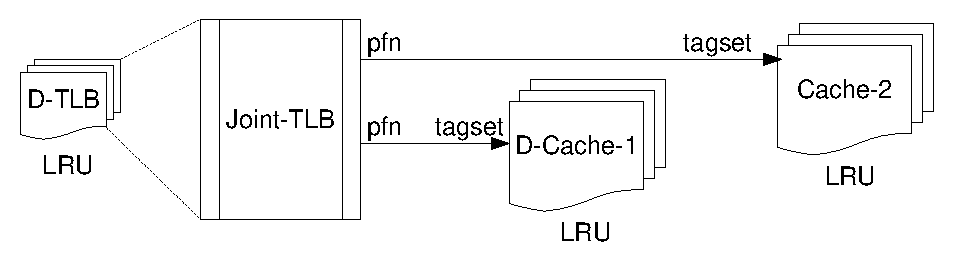
\includegraphics[width=0.8\textwidth]{4.analysis/mips}\\
  \caption{Схема MMU микропроцессора MIPS}\label{mips_mmu_scheme}
\end{figure}

По шагам подготовки генератора тестовых программ:
\begin{enumerate}
  \item\label{step_mmu} структура MMU построена, для этого пришлось ознакомиться с
  документацией по архитектуре микропроцессора~\cite{mips64_III},
  это заняло 1 человеко-день;
  \item\label{step_procedures}
  на основе анализа системы команд архитектуры MIPS~\cite{mips64_II}
  были выделены следующие процедуры для описания тестовых
  ситуаций:\\
  AddressTranslation, LoadMemory, StoreMemory, BytesSelect,
  BytesExpand -- на это ушел 1 человеко-день;
  \item в генераторе ограничений был использован зеркальный метод
  генерации ограничений для кэшируемых неотображаемых обращений и
  совместно-зеркальный метод генерации ограничений для остальных
  обращений -- на это ушло с учетом отладки 5 человеко-дней;
  \item для процедуры AddressTranslation в виде ограничений была
  записана модель виртуальной памяти (виды обращений в разных
  областях виртуальной памяти -- кэшируемое или некэшируемое,
  отображаемое или неотображаемое), для процедуры LoadMemory в виде
  ограничений были записаны взаимосвязи физических адресов и
  считанных из основной памяти данных (см.
  п.~\ref{module_algorithm} диссертации), для процедур BytesSelect и
  BytesExpand был выписан перебор значений младших бит физического
  адреса и границ части нужной длины двойного слова, являющего
  результатом чтения из памяти или записи в память -- с учетом
  отладки на это ушло 3 человеко-дня;
  \item\label{step_testsituations}
   по результатам знакомства с документацией по системе команд
  архитектуры MIPS~\cite{mips64_II} было выделено 8 инструкций
  (load / store --- byte / halfword / word / doubleword), в каждой инструкции по
  2 тестовые ситуации (AddressError(невыровненный виртуальный
  адрес) / полное выполнение инструкции), на подготовку описаний
  тестовых ситуаций ушло 1 человеко-день;
  \item\label{step_z3} использовался решатель ограничений Z3~\cite{Z3}, который
  печатал модель в виде пар <<(имя, значение)>>, среди имен
  выбирались начальные значения регистров и инициализирующие тегсеты
  кэшируемых неотображаемых обращений, по которым генерировались
  инициализирующие инструкции -- с учетом отладки на это ушло 1
  человеко-день;
  \item\label{step_compose} были объединены имеющиеся компоненты чтения описаний
  тестовых ситуаций и построения ограничений для операторов
  \texttt{let} и \texttt{assert} и новые компоненты, описывающие
  последовательности тестовых ситуаций в кэш-памяти и TLB,
  описывающие процедуры описаний тестовых ситуаций и генерирующие
  искомую тестовую программу -- на это ушло 1 человеко-день.
\end{enumerate}

Итого на построение генератора тестовых программ для MIPS ушло около
2,5 человеко-недель. При этом при построении генератора тестовых
программ для другого микропроцессора архитектуры MIPS (он может
отличаться количественными параметрами кэширующих буферов, размерами
виртуальных и физических адресов) повторно можно использовать
результаты шагов \ref{step_mmu}, \ref{step_procedures},
\ref{step_testsituations}, \ref{step_z3} и \ref{step_compose},
остальные шаги выполняются аналогичным образом с заменой
количественных параметров . Это позволяет достичь уровень
переиспользования в 40\% ($\frac{5 * 100\%}{13}$). Ручное создание
генератора тестовой программы для микропроцессора MIPS RM7000
~\cite{kamkin} заняло в сумме 2 человеко-месяца. Данные о
трудоемкости показывают, что при сходной полноте тестового набора
представленные в диссертации методы позволяют сократить время
построения генератора тестовых программ более чем в 3 раза.

Был подготовлен прототип генератора тестовых программ для
микропроцессора архитектуры MIPS. Были проведены эксперименты по
генерации тестовых программ на массивах тестовых шаблонов. Первый
набор экспериментов был связан с исследованием вероятности того, что
ограничения, построенные по методу совместной генерации, будут
совместны и дадут искомую тестовую программу. В таблице~\ref{exps1}
приведены результаты этих экспериментов для тестовых шаблонов из
двух инструкций. Таких тестовых шаблонов с различными
неэквивалентными зависимостями по данным было 240. Из них 15\%
несовместных тестовых шаблонов (для них не может существовать ни
одна тестовая программа). Остальные 85\% тестовых шаблонов составили
основу экспериментов. Были подготовлены начальные состояния
микропроцессора двух типов: произвольные (значения тегов в ячейках
кэш-памяти были сгенерированы случайным образом) и подготовленные
(значения тегов в ячейках были выбраны так, чтобы они с большей
вероятностью пересекались с номерами физических кадров состояния
TLB).

\begin{table}[h]
  \begin{tabular}{|c|c|c|c|c|}
  \hline
  \begin{tabular}{c}тип\\начального\\состояния\end{tabular}&
  \begin{tabular}{c}доля\\реали-\\зованных\\тестовых\\шаблонов\end{tabular}&
  \begin{tabular}{c}доля\\нереализо-\\ванных\\тестовых\\шаблонов\end{tabular}&
  \begin{tabular}{c}КПД\\совместной\\генерации\end{tabular}&
  \begin{tabular}{c}общее\\время\\генерации\end{tabular}\\
  \hline \hline
  подготовленное & 49~\% & 36~\% & 58~\% & 85~с. \\
  \hline
  произвольное & 32~\% & 53~\% & 38~\% & 170~с. \\
  \hline
  \end{tabular}
  \caption{Эксперименты с совместной генерацией; $n$ =
  2}\label{exps1}
\end{table}

Эксперименты показали, что использование совместной генерации на
произвольных начальных данных дает возможность построить тестовые
программы для 35-40\% тестовых шаблонов с различными зависимостями
по регистрам; на подготовленных начальных данных применением
совместной генерации удается достичь 55-60\% покрытия для тестовых
шаблонов. Важны оба случая, поскольку при первом запуске состояние
микропроцессора будет произвольным, а при всех последующих запусках
состояния, полученных от прошлых запусков, будут уже подготовленными
--- тем самым повысится вероятность построения тестовой программы по
ограничениям, сгенерированным методом совместной генерации.
Зеркальным методом (в силу его полноты) удалось построить тестовые
программы для всех тестовых совместных шаблонов. На все тестовые
шаблоны <<зеркальному методу>> потребовалось около 220 секунд.

%% посмотреть n = 3 и n = 4

%% посмотреть максимальную длину минимальной необходимой длины
%% инициализирующей последовательности для зеркальной генерации

\section{Генерация ограничений для архитектуры PowerPC}

\begin{utv}
Для архитектуры PowerPC возможно применение применение методов
генерации ограничений, описыванных в диссертации, для генерации
тестовых программ по тестовым шаблонам; причем методов достаточно
для полного описания поведения MMU микропроцессоров архитектуры
PowerPC.
\end{utv}

Рассмотрим исполнение инструкции обращения к памяти в
микропроцессоре архитектуры PowerPC~\cite{shnitman}. MMU в
микропроцессорах PowerPC включает в себя (количественные
характеристики приведены для микропроцессора PowerPC 970FX
~\cite{PowerPC970FXUserManual} -- см.
рис.~\ref{powerpc_mmu_scheme}):
\begin{itemize}
  \item \emph{кэш-память данных первого уровня (D-Cache-1)}: размер 32
килобайта, наборно-ассоциативная кэш-память, количество секций равно
2, размер строки кэш-памяти 128 байт, effective index real tag,
стратегия вытеснения \LRU;
  \item \emph{кэш-память второго уровня (Cache-2)}: размер 512
  килобайт, наборно-ассоциативная кэш-память, количество секций
  равно 8, стратегия вытеснения LRU, размер строки кэш-памяти 128
  байт, real index real tag;
  \item \emph{кэш-буфер TLB (D-TLB)}: наборно-ассоциативный буфер,
  количество секций 4, количество наборов в каждой секции 256;
  стратегия вытеснения LRU;
  \item \emph{таблица страниц виртуальной памяти (PageTable)}: размер
  виртуального адреса 65 бит, размер физического адреса 42 бита;
  \item \emph{сегментные регистры (SLB)}: полностью ассоциативный
  буфер, размер 64 строки;
  \item \emph{буфер непосредственной трансляции адресов (D-ERAT)}:
  наборно-ассоциативный буфер, количество секций равно 2, в каждой
  секции по 64 строки; стратегия вытеснения \FIFO.
\end{itemize}
Таким образом, проблема возникнет при записи ограничений на
кэш-память и на TLB.

Инструкция может содержать тестовые ситуации в:
\begin{itemize}
  \item кэш-памяти данных первого уровня, первого и второго уровней;
  \item кэш-буфере данных TLB (D-TLB);
  \item кэш-буфере непосредственной трансляции адресов (D-ERAT).
\end{itemize}

\begin{figure}[h] \center
  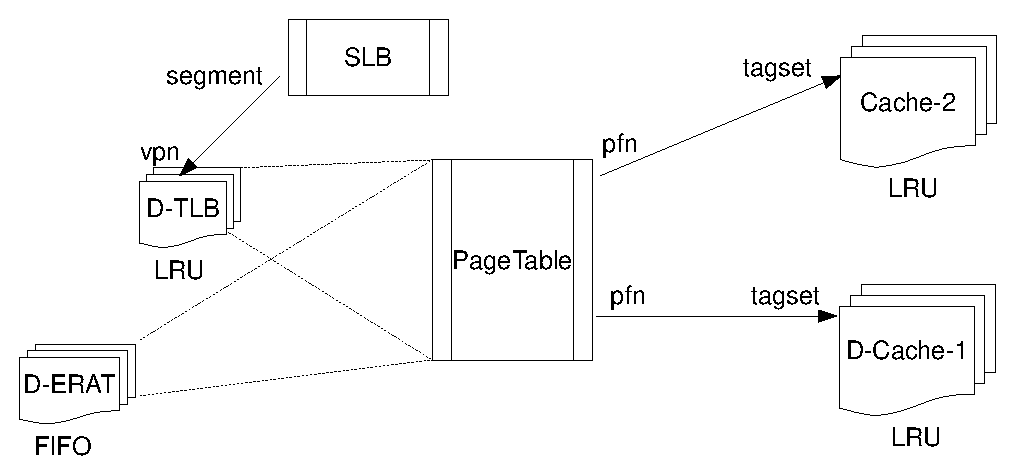
\includegraphics[width=0.8\textwidth]{4.analysis/ppc}\\
  \caption{Схема MMU микропроцессора PowerPC 970FX}\label{powerpc_mmu_scheme}
\end{figure}

Совместная генерация возможна (см. рис.~\ref{powerpc_mmu_scheme}):
\begin{itemize}
  \item на границе D-ERAT--кэш-память, так как получаемый из D-ERAT номер
физического кадра (pfn) становится битовым полем тегсета физического
адреса;
  \item на границе SLB--D-TLB, так как значение сегментного регистра
  становится битовым полем номера страницы виртуальной памяти (vpn);
  \item на границе D-TLB--кэш-память, так как получаемый из D-TLB номер
физического кадра (pfn) становится битовым полем тегсета физического
адреса.
\end{itemize}

\section{Генерация ограничений для архитектуры Alpha}

\begin{utv}
Для архитектуры Alpha возможно применение применение методов
генерации ограничений, описыванных в диссертации, для генерации
тестовых программ по тестовым шаблонам.
\end{utv}

Рассмотрим исполнение инструкции обращения к памяти в
микропроцессоре архитектуры Alpha. MMU в микропроцессорах Alpha
включает в себя  (количественные характеристики приведены для
микропроцессора Alpha 21264~\cite{HennessyPatterson3rd} -- см.
рис.~\ref{alpha_mmu_scheme}):
\begin{itemize}
  \item \emph{кэш-память данных первого уровня (D-Cache-1)}:
  virtually indexed physically tagged, размер 64 килобайта,
  наборно-ассоциативный, количество секций равно 2, стратегия вытеснения
  \LRU, размер строки кэш-памяти 64 байта;
  \item \emph{кэш-память второго уровня (Cache-2)}: physically
  indexed physically tagged, прямого отображения, размер от 1 до 16
  мегабайт
  \item \emph{таблица TLB (D-TLB)}: 128 строк, полностью
  ассоциативная, размер виртуального адреса 48/43 бит, размер физического адреса
  44/41 бит, размер страницы виртуальной памяти от 8 килобайт до 4
  мегабайт;
  \item \emph{буфер вытесненных данных (VictimBuffer)}: полностью
  ассоциативный, количество строк равно 8, стратегия
  вытеснения \FIFO.
\end{itemize}
Таким образом, основная проблема при записи ограничений -- большой
размер содержимого кэш-памяти.

Инструкция может содержать тестовые ситуации в:
\begin{itemize}
  \item кэш-памяти данных первого уровня;
  \item кэш-памяти первого и второго уровней.
\end{itemize}

\begin{figure}[h] \center
  \includegraphics[width=0.8\textwidth]{4.analysis/alpha}\\
  \caption{Схема MMU микропроцессора Alpha}\label{alpha_mmu_scheme}
\end{figure}

Совместная генерация возможна на границе TLB--кэш-память, так как
получаемый из TLB номер физического кадра (pfn) становится битовым
полем тегсета физического адреса (см.рис.~\ref{alpha_mmu_scheme}).



\section{Генерация ограничений для архитектуры Pentium}

\begin{utv}
Для архитектуры Pentium возможно применение применение методов
генерации ограничений, описыванных в диссертации, для генерации
тестовых программ по тестовым шаблонам.
\end{utv}

Рассмотрим исполнение инструкции обращения к памяти в
микропроцессоре архитектуры Pentium P6. MMU в микропроцессорах
Pentium включает в себя (количественные характеристики приведены для
микропроцессора Intel Pentium III~\cite{HennessyPatterson3rd} -- см.
рис.~\ref{p6_mmu_scheme}):
\begin{itemize}
  \item \emph{кэш-память данных первого уровня (D-Cache-1)}: размер
  16 килобайт, наборно-ассоциативная, количество секций равно 2,
  стратегия вытеснения \LRU, размер строки 32 байта;
  \item \emph{кэш-память второго уровня (Cache-2)}: размер от 256 килобайт
  до 2 мегабайт, наборно-ассоциативная, количество секций равно 8, стратегия
  вытеснения \LRU, размер строки 32 байта;
  \item \emph{кэш-буфер TLB (D-TLB)}: наборно-ассоциативный,
  количество секций равно 4, в каждой секции 16 строк, стратегия вытеснения
  \PseudoLRU;
  \item \emph{таблица страниц виртуальной памяти (PageTable)}:
  размер страницы от 8 килобайт, длина логического адреса 48 бит,
  длина линейного адреса 32 бита, длина физического адреса 32 бита;
  \item \emph{таблица дескрипторов сегментов (SDT)}: размер от 8 байт до 64
  килобайт~\cite{FundamentalOfComputerOrganizationAndDesign}.
\end{itemize}
Таким образом, проблема возникнет при записи ограничений на
кэш-память и на TLB.

Инструкция может содержать тестовые ситуации в:
\begin{itemize}
  \item кэш-памяти данных первого уровня, первого и второго уровней;
  \item кэш-буфере данных TLB (D-TLB).
\end{itemize}

\begin{figure}[h] \center
  \includegraphics[width=0.8\textwidth]{4.analysis/p6}\\
  \caption{Схема MMU микропроцессора Pentium}\label{p6_mmu_scheme}
\end{figure}

Совместная генерация возможна (см. рис.~\ref{p6_mmu_scheme}):
\begin{itemize}
  \item на границе SDT--D-TLB, так как значение сегментного регистра
  становится битовым полем номера страницы виртуальной памяти (vpn);
  \item на границе D-TLB--кэш-память, так как получаемый из D-TLB номер
физического кадра (pfn) становится битовым полем тегсета физического
адреса;
  \item на границе SDT--кэш-память при неотображаемом обращении, так как
  получаемый из SDT сегментный регистр становится битовым полем тегсета физического
адреса.
\end{itemize}
